\documentclass{beamer}

\usepackage[utf8]{inputenc}
\usepackage{fancybox}
\usepackage{environ}
\usepackage{tikz}

\beamertemplatenavigationsymbolsempty
\setbeamertemplate{footline}[frame number]

\title{2.1 Solution Curves (Without a Solution)}

\subtitle{a lesson for MATH F302 Differential Equations}

\author{Ed Bueler, Dept.~of Mathematics and Statistics, UAF}

\date{\tiny \today}


\usetheme{Pittsburgh}


\begin{document}

\setbeamertemplate{itemize item}{$\bullet$}
\setbeamertemplate{itemize subitem}{$\circ$}


\begin{frame}
\titlepage

\centerline{\tiny for textbook: \, D. Zill, \emph{A First Course in Differential Equations with Modeling Applications}, 11th ed.}
%\color{green!40!blue}
\end{frame}


\begin{frame}{meaning of a differential equation}

\begin{itemize}
\item start over on the meaning of a (first-order) DE:
    $$\frac{dy}{dx} = f(x,y)$$

\vspace{-2mm}
    \begin{enumerate}
    \item the left side is the \emph{slope} of the solution $y(x)$
    \item given a pair $(x,y)$, the right side computes a number $f(x,y)$
    \end{enumerate}
\item thus a differential equation \emph{is} a statement:
    $$\begin{matrix}
    \text{the slope of the} \\
    \text{solution } y(x) 
    \end{matrix} \quad \stackrel{\text{equals}}{=} \quad
    \begin{matrix}
    \text{a known function of} \\
    \text{the location } (x,y)
    \end{matrix}$$
\item this literal reading of the DE means that

\centerline{\alert{we can \emph{draw} a picture of the DE itself}}

\item \dots whether or not we can do the calculus/algebra to find a formula for $y(x)$
\end{itemize}
\end{frame}


\begin{frame}{direction field}

\begin{itemize}
\item again, $\frac{dy}{dx} = f(x,y)$ should be read as a way of computing a slope ($dy/dx$) at each location in the plane ($(x,y)$)
\item you can create a \emph{direction field} or \emph{slope field}:
    \begin{enumerate}
    \item generate a grid of point in the $x$--$y$ plane
    \item for each point, draw a short line with the slope given by $f(x,y)$ at that point
    \end{enumerate}
\item see also: \small \href{https://en.wikipedia.org/wiki/Slope_field}{\color{blue} \texttt{en.wikipedia.org/wiki/Slope\_field}} \normalsize

\bigskip
\item \begin{minipage}[t]{0.375\textwidth}
\emph{Example.}  By hand, draw a direction field for
$$\frac{dy}{dx} = x-y$$
on the square
$$-3 \le x \le 3, -3 \le y \le 3$$
\end{minipage} 

\vspace{20mm}
\end{itemize}
\end{frame}


\begin{frame}{a computer is wanted}

\begin{itemize}
\item o.k., I acknowledge \emph{happily} that this is a job for a computer
\item see ``found online'' at the \href{https://bueler.github.io/math302/week2.html}{\color{blue} Week 2 tab}
\item \emph{Example.}  Use a computer to draw a direction field for
$\frac{dy}{dx} = x-y$ on the square $-3 \le x \le 3, -3 \le y \le 3$

\bigskip
\emph{Solution}:

\vspace{-5mm}
\hfill 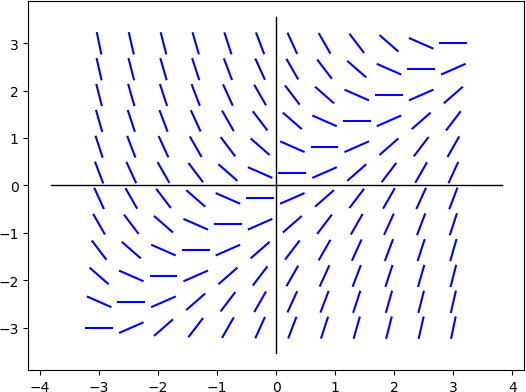
\includegraphics[width=0.5\textwidth]{figs/example-field}
\end{itemize}
\end{frame}


\begin{frame}{picturing ODE IVPs}

\begin{itemize}
\item recall that we are often solving initial value problems
\item one can \emph{see} the solution in the direction field

\bigskip
\item \begin{minipage}[t]{0.37\textwidth}
\emph{Example.}  Use the direction field for
$\frac{dy}{dx} = x-y$ to sketch the solution of
    $$\frac{dy}{dx} = x-y, \quad y(0)=2$$
\end{minipage}

\vspace{-25mm}
\hfill 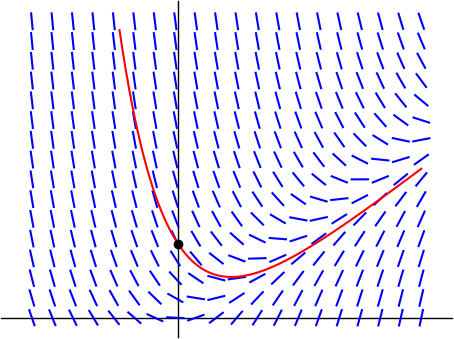
\includegraphics[width=0.5\textwidth]{figs/example-field-solution}
\end{itemize}
\end{frame}


\begin{frame}{X}

\begin{itemize}
\item X
\end{itemize}
\end{frame}


\begin{frame}{X}

\begin{itemize}
\item X
\end{itemize}
\end{frame}


\begin{frame}{X}

\begin{itemize}
\item X
\end{itemize}
\end{frame}


\begin{frame}{X}

\begin{itemize}
\item X
\end{itemize}
\end{frame}


\begin{frame}{X}

\begin{itemize}
\item X
\end{itemize}
\end{frame}




\begin{frame}{expectations}

to learn this material, just watching this video is \emph{not} enough; also
\begin{itemize}
\item \emph{read} section 2.1 in the textbook
\item \emph{do} the WebAssign exercises for section 2.1
\item see the other ``found online'' videos at bottom of this page:

\centerline{\href{https://bueler.github.io/math302/week2.html}{\tt \color{cyan} bueler.github.io/math302/week2.html}}
\end{itemize}
\end{frame}

\end{document}

